\documentclass[compress]{beamer}        % [compress] (written before {beamer} <=> navigation bar one line, all subsections in 1 line instead of 2

% Setup appearance:
\usetheme{CambridgeUS}
%	AnnArbor | Antibes | Bergen |
%	Berkeley | Berlin | Boadilla |
%	boxes | CambridgeUS | Copenhagen |
%	Darmstadt | default | Dresden |
%	Frankfurt | Goettingen |Hannover |
%	Ilmenau | JuanLesPins | Luebeck |
%	Madrid | Malmoe | Marburg |
%	Montpellier | PaloAlto | Pittsburgh |
%	Rochester | Singapore | Szeged |
%	Warsaw
%

\useoutertheme[footline=authorinstitute,subsection=false]{miniframes}
\usecolortheme{whale}

%	albatross | beaver | beetle |
%	crane | default | dolphin |
%	dove | fly | lily | orchid |
%	rose |seagull | seahorse |
%	sidebartab | structure |
%	whale | wolverine


\setbeamertemplate{footline}
{
  \hbox{%
  \begin{beamercolorbox}[wd=.25\paperwidth,ht=2.25ex,dp=1ex,center]{title in head/foot}%
    \usebeamerfont{date in head/foot}\insertshortauthor
  \end{beamercolorbox}%
  \begin{beamercolorbox}[wd=.5\paperwidth,ht=2.25ex,dp=1ex,center]{date in head/foot}%
    \usebeamerfont{title in head/foot}\insertshortinstitute
  \end{beamercolorbox}%
  \begin{beamercolorbox}[wd=.25\paperwidth,ht=2.25ex,dp=1ex,center]{title in head/foot}%
    \usebeamerfont{date in head/foot}
    \insertframenumber{} / \inserttotalframenumber
  \end{beamercolorbox}}%
  \vskip0pt%
}

%\setbeamercolor{titlelike}{parent=structure}
%\setbeamercolor{structure}{fg=beamer@blendedblue}
%% \useinnertheme{rounded}
%\setbeamerfont{block title}{size={}}
%\usefonttheme[onlylarge]{structurebold}   % title and words in the table of contents bold
%\setbeamerfont*{frametitle}{size=\normalsize,series=\bfseries}
\setbeamertemplate{navigation symbols}{}
\setbeamercolor{frametitle}{parent=boxes, bg=white}


% Standard packages

\usepackage[english]{babel}
\usepackage[latin1]{inputenc}
\usepackage{times}
\usepackage[T1]{fontenc}
\usepackage{amsbsy}         % for \boldsymbol command (bold in math mode)
\usepackage{amsfonts, amssymb}
\usepackage{epsfig}
\usepackage{color}
\definecolor{camblue}{RGB}{26,26,89}
\definecolor{Rblue}{RGB}{0,255,255}
\definecolor{Rdarkblue}{RGB}{0,0,255}
\definecolor{Rgreen}{RGB}{0,205,0}
\newcommand{\tcb}{\textcolor{beamer@blendedblue}}
\newcommand{\tcbb}{\textcolor{camblue}}
\newcommand{\tcr}{\textcolor{red}}
\newcommand{\tcg}{\textcolor{gray}}
\newcommand{\tcRg}{\textcolor{Rgreen}}
\newcommand{\tcRdb}{\textcolor{Rdarkblue}}
\newcommand{\tcRb}{\textcolor{Rblue}}
\newcommand{\sq}{\begin{eqnarray}}
\newcommand{\fq}{\end{eqnarray}}
\newcommand{\bp}{$\bullet$\:}


%%%%%%%%%%%%%%%%%%%%%%%%%%%%%%%%%%%%%%%%%%%%%%%%%%%%%%%%%%%%%%%%%%%%%%%%%%%%%%%%%%%%%%%%%%%%%
% THIS IS WHERE THE DOCUMENT BEGINS


%\setbeamercovered{transparent}   % overlays with light grey 1st slide
\title
{
{\huge Title\\[0.3cm] }
}
\author[Kevin O'Brien]{{\bf Author}}
\institute[University of Limerick, Maths \& Stats Dept]{}
\date{}

\begin{document}

\begin{frame}
\huge
\[ \mbox{Method Comparison Studies with \texttt{R}} \]
\Large
\[ \mbox{Kevin O'Brien} \]
\end{frame}
\begin{frame}
\setcounter{tocdepth}{1}
\tableofcontents
\end{frame}

%------------------------------------------------------------------------%
\section[Intro to MCS]{Introduction to Method Comparison Studies}
\subsection{Method Comparison Studies}
%\begin{frame}{\bf \tcb{Intro}}
%\begin{itemize}\itemsep0.7cm
%\item Commonly encountered issue in medical statistics
%\item ``Do two methods of measurement agree statistically?".
%\item ``Can the two methods be used interchangeably?"
%\item Sources of disagreement can arise from differing population means (i.e. inter-method bias), differing between-subject and with-in subject variances \cite{Roy2009}.
%\end{itemize}
%\end{frame}
%---------------------------------------------%
\begin{frame}
\large
\vspace{-1cm}
\textbf{Method Comparison Studies}
\begin{itemize}
\item The problem of assessing the \textbf{agreement} between two or more methods
of measurement is ubiquitous in scientific research, particularly with clinical sciences, and is
commonly referred to as a `method comparison study'. 
{
\large
\begin{itemize}
\item ``Do two methods of measurement agree statistically?".
\item ``Can the two methods be used interchangeably?"
\end{itemize}
}

\item Published
examples of method comparison studies can be found in disciplines
as diverse as Pharmacology \alert{ludbrook97}, Anaesthesia
\alert{Myles}, and cardiac imaging methods \alert{Krumm}

\end{itemize}


\end{frame}

%---------------------------------------------%
\begin{frame}
\frametitle{Accuracy and Precision}
\large
\begin{itemize}
\item
A method of measurement should ideally be both accurate and
precise. 
\item \alert{Barnhart} describes agreement as being a broader
term that contains both of those qualities. An accurate
measurement method will give results close to the unknown `true
value'. \item The precision of a method is indicated by how tightly
measurements obtained under identical conditions are distributed
around their mean measurement value.\item A precise and accurate method
will yield results consistently close to the true value. 
\end{itemize}
\end{frame}
%---------------------------------------------%
\begin{frame}
\frametitle{Accuracy and Precision}
\large
\begin{itemize}
\item Of course
a method may be accurate, but not precise, if the average of its
measurements is close to the true value, but those measurements
are highly dispersed. 
\item
Conversely a method that is not accurate may
be quite precise, as it consistently indicates the same level of
inaccuracy. 
\item The tendency of a method of measurement to
consistently give results above or below the true value is a
source of systematic bias. 
\item The smaller the systematic bias, the
greater the accuracy of the method.
\end{itemize}
\end{frame}
%---------------------------------------------%
\begin{frame}
\frametitle{Accuracy and Precision}
%\frametitle{Method Comparison Studies with \texttt{R}}
\large
\begin{itemize}
\item 
The FDA define precision as the closeness of agreement (degree of
scatter) between a series of measurements obtained from multiple
sampling of the same homogeneous sample under prescribed
conditions. \item \alert{Barnhart} describes precision as being further
subdivided as
\begin{enumerate}
\item  within-run, intra-batch precision or
repeatability (which assesses precision during a single analytical
run), 
\item between-run, inter-batch precision or repeatability
(which measures precision over time)
\end{enumerate} 
\end{itemize}
\end{frame}
%---------------------------------------------%
\begin{frame}
\frametitle{Inter-Method Bias}
\large
\vspace{-1cm}
\begin{itemize}
\item 
In the context of the agreement of two methods, there is also a
tendency of one measurement method to consistently give results
above or below the other method. \item Lack of agreement is a
consequence of the existence of `inter-method bias'. 
\item For two
methods to be considered in good agreement, the inter-method bias
should be in the region of zero. 
\end{itemize}
\end{frame}
%---------------------------------------------%
\begin{frame}
\frametitle{Inter-Method Bias}
\large
\begin{itemize}
\item 
A simple estimation of the
inter-method bias can be calculated using the differences of the
paired measurements. \item The data in Table 1.2 (\textit{next slide}) are a good example of
possible inter-method bias; the `Fotobalk' consistently recording
smaller velocities than the `Counter' method.
\item Consequently one
would conclude that there is lack of agreement between the two
methods.
\end{itemize}
\end{frame}
%------------------------------------------------------------------ %
\subsection*{Systematic and random errors}
\begin{frame}
% MA4605 Notes
Experimental scientists make a fundamental distinction between \textbf{\emph{random}}, and
 \textbf{\emph{systematic}} errors. To distinguish between random and systematic errors let
us consider a real experiment.\\

\noindent Four students (A-D) each perform an analysis in which exactly 10.00 $ml$
of exactly 0.1 M sodium hydroxide is titrated with exactly 0.1 NI
hydrochloric acid.
Each student performs five replicate titrations, with the results shown in
Table 1.1.
\end{frame}
%------------------------------------------------------------------ %
\begin{frame}
% MA4605 Notes
\begin{tabular}{|c|ccccc|l|}
  \hline
  % after \\: \hline or \cline{col1-col2} \cline{col3-col4} ...
Student & Results  & (ml) &  &  &  &Comment \\ \hline
A & 10.08 & 10.11 &10.09 &10.10&10.12 & Precise, biased\\ \hline
B & 9.88 &10.14& 10.02 &9.80& 10.21& Imprecise unbiased\\ \hline
C & 10.19 &9.79& 9.69 &10.05& 9.78 & Imprecise, biased\\ \hline
D & 10.04 &9.98 &10.02 &9.97 &10.04 & Precise, unbiased \\
  \hline
\end{tabular}
\bigskip
\end{frame}
%------------------------------------------------------------------ %
\begin{frame}
% MA4605 Notes
\textbf{Graphical illustration}


The results of experiment represented by dot-plots. (The true value is 10.00).

\begin{center}
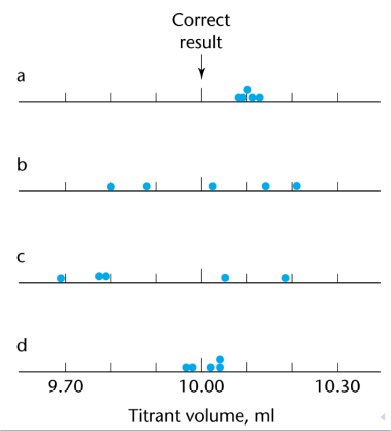
\includegraphics[scale=0.6]{Image10}
\end{center}
\end{frame}
%------------------------------------------------------------------ %
\begin{frame}
% MA4605 Notes
Recall the average for each student $ 10.0950, 9.9600, 9.9300, 10.0025 $ respectively.
\newpage

\textbf{Systematic error and bias}\\
Systematic error is a deviation of all measurements in one direction from the true value. It is well represented by the difference between the average value of the determined values and the true value
of the measured quantity. This difference is called the bias of measurements.

\textbf{Random error and precision}\\
Random error is a deviation of a measurement from the average of measured values.
It is well represented by the standard deviation of measurements.
This value is often called precision of measurements.

\textbf{Combined error vs. accuracy}\\
Accuracy is in inverse relation to the total deviation of a single measurement from the true value.
\end{frame}
%------------------------------------------------------------------------%

\begin{frame}{\bf \tcb{Three Conditions}}
For two methods of measurement to be considered interchangeable, the following conditions must apply \cite{Roy2009}:
\\
\begin{itemize}\itemsep0.5cm
\item No significant inter-method bias
\item No difference in the between-subject variabilities of the two methods
\item No difference in the within-subject variabilities of the two methods (repeatability)
\end{itemize}
\end{frame}



%---------------------------------------------%
\subsection{Grubbs Example}
%---------------------------------------------%
\begin{frame}
\large
\vspace{-1cm}
\begin{itemize}
\item To illustrate the characteristics of a typical method comparison
study consider the data in Table I  \alert{Grubbs73}. 
\item 


In each of
twelve experimental trials a single round of ammunition was fired
from a 155mm gun, and its velocity was measured simultaneously
(and independently) by three chronographs devices, identified here
by the labels `\textbf{\textit{Fotobalk}}', `\textbf{\textit{Counter}}' and `\textbf{\textit{Terma}}'.
\end{itemize}
\end{frame}
%---------------------------------------------%
\begin{frame}
\large

\begin{table}[ht]
\begin{center}
\begin{tabular}{rrrr}
  \hline
  Round& Fotobalk [F] & Counter [C]& Terma [T]\\
  \hline
  1 & 793.8 & 794.6 & 793.2 \\
  2 & 793.1 & 793.9 & 793.3 \\
  3 & 792.4 & 793.2 & 792.6 \\
  4 & 794.0 & 794.0 & 793.8 \\
  5 & 791.4 & 792.2 & 791.6 \\
  6 & 792.4 & 793.1 & 791.6 \\
  7 & 791.7 & 792.4 & 791.6 \\
  8 & 792.3 & 792.8 & 792.4 \\
  9 & 789.6 & 790.2 & 788.5 \\
  10 & 794.4 & 795.0 & 794.7 \\
  11 & 790.9 & 791.6 & 791.3 \\
  12 & 793.5 & 793.8 & 793.5 \\
   \hline
\end{tabular}
\caption{Velocity measurement from the three chronographs (Grubbs
1973).}
\end{center}
\end{table}
\end{frame}
%---------------------------------------------%
\begin{frame}
\large
\begin{itemize}
\item An important aspect of the these data is that all three methods of
measurement are assumed to have an attended \textbf{\textit{measurement error}}, and
the velocities reported in Table 1.1 can not be assumed to be
`true values' in any absolute sense.
\end{itemize}


%While lack of
%agreement between two methods is inevitable, the question , as
%posed by \alert{BA83}, is 'do the two methods of measurement agree
%sufficiently closely?'
\end{frame}
%---------------------------------------------%
\begin{frame}
\large
% latex table generated in R 2.6.0 by xtable 1.5-5 package
% Wed Aug 26 15:22:41 2009
\begin{table}[h!]

\begin{center}

\begin{tabular}{rrrr}
  \hline
 Round& Fotobalk (F) & Counter (C) & F-C \\
  \hline
1 & 793.8& 794.6 & -0.8 \\
  2 & 793.1 & 793.9 & -0.8 \\
  3 & 792.4 & 793.2 & -0.8 \\
  4 & 794.0 & 794.0 & 0.0 \\
  5 & 791.4 & 792.2 & -0.8 \\
  6 & 792.4 & 793.1 & -0.7 \\
  7 & 791.7 & 792.4 & -0.7 \\
  8 & 792.3 & 792.8 & -0.5 \\
  9 & 789.6 & 790.2 & -0.6 \\
  10 & 794.4 & 795.0 & -0.6 \\
  11 & 790.9 & 791.6 & -0.7 \\
  12 & 793.5 & 793.8 & -0.3 \\
   \hline
\end{tabular}
\caption{Difference between Fotobalk and Counter measurements.}
\end{center}
\end{table}
\end{frame}




%------------------------------------------------------------------------%
\section{Bland-Altman Methods}

\begin{frame}
\frametitle{Bland-Altman Methods}
\large
\textbf{Section 2 - Bland-Altman Methods}
\begin{itemize}
\item Bland-Altman's Methods
\item Limits of Agreement
\item Implementation with \texttt{R}
\item Other R Packages
\end{itemize}
\end{frame}

%------------------------------------------------------------------------%

\begin{frame}{\bf \tcb{The Bland-Altman Plot}}
\begin{itemize}\itemsep0.7cm

\item The Bland-Altman plot \cite{BA86,BA99} is a very simple graphical method to compare two measurements techniques. \item In this approach the case-wise differences between the two methods are plotted against the corresponding case-wise averages of the two methods.

\item A horizontal lines is drawn at the mean difference(the inter-method bias) , and at the limits of agreement, which are defined as the inter-method bias plus and minus 2 times the standard deviation of the differences.
\end{itemize}
\end{frame}












%%%%%%%%%%%%%%%%%%%%%%%%%%%%%%%%%%%%%%%%%%%%%%%%%%%%%%%%%%%%%%%%%%%%%%%%%%%%%%%%%%%%%%

\subsection{Bland-Altman Difference Plot}
\begin{frame}
\frametitle{Bland-Altman Plots}
\large
\begin{itemize}
\item 
The issue of whether two measurement methods comparable to the
extent that they can be used interchangeably with sufficient
accuracy is encountered frequently in scientific research.
\item Historically comparison of two methods of measurement was carried
out by use of paired sample t-test, correlation coefficients or
simple linear regression.
\item  Statisticians Martin Bland and Douglas
Altman recognized the inadequacies of these analyses and
articulated quite thoroughly the basis on which of which they are
unsuitable for comparing two methods of measurement \alert{BA83}.

\end{itemize}
\end{frame}
%%%%%%%%%%%%%%%%%%%%%%%%%%%%%%%%%%%%%%%%%%%%%%%%%%%%%%%%%%%%%%%%%%%%%%%%%%%%%%%%%%%%%%
\begin{frame}
\frametitle{Bland-Altman Plots}
\large
\begin{itemize}
\item 
Furthermore they proposed their simple methodology specifically
constructed for method comparison studies. 
\item They acknowledge the
opportunity to apply other valid, but complex, methodologies, but
argue that a simple approach is preferable, especially when the
results must be `\textit{explained to non-statisticians}'.
\end{itemize}
\end{frame}
%%%%%%%%%%%%%%%%%%%%%%%%%%%%%%%%%%%%%%%%%%%%%%%%%%%%%%%%%%%%%%%%%%%%%%%%%%%%%%%%%%%%%%
\begin{frame}
\frametitle{Bland-Altman Plots}
\large
\begin{itemize}
\item Notwithstanding previous remarks about regression, the first step
recommended, which the authors argue should be mandatory, is
construction of a simple scatter plot of the data. 
\item The \textbf{\textit{line of
equality}} must also be shown, as it is necessary to give the
correct interpretation of how both methods compare. 
\item A scatter plot
of the Grubbs data is shown in Figure 1.1. 
\item Visual inspection confirms the previous conclusion that there is an
inter-method bias present, i.e. Fotobalk device has a tendency to
record a lower velocity.
\end{itemize}
\end{frame}
%%%%%%%%%%%%%%%%%%%%%%%%%%%%%%%%%%%%%%%%%%%%%%%%%%%%%%%%%%%%%%%%%%%%%%%%%%%%%%%%%%%%%%
\begin{frame}
\begin{figure}[h!]
\begin{center}
  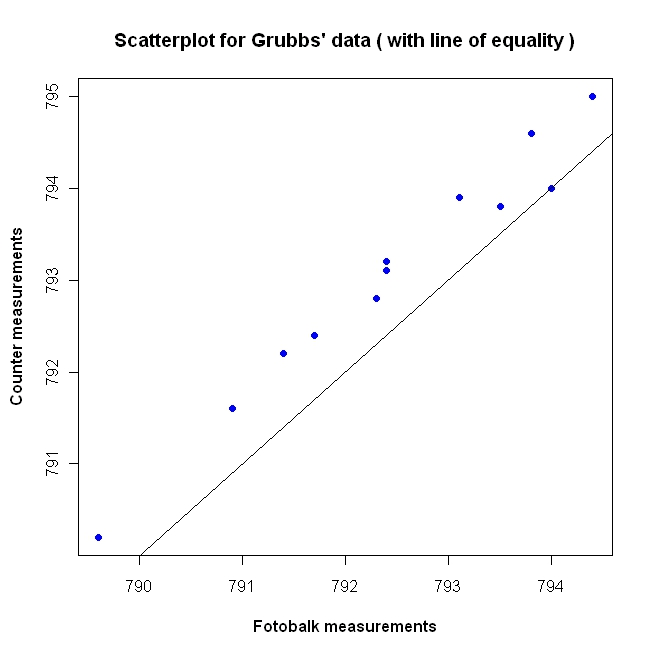
\includegraphics[width=80mm]{GrubbsScatter.jpeg}
  \caption{Scatter plot For Fotobalk and Counter Methods.}\label{GrubbsScatter}
\end{center}
\end{figure}
\end{frame}
%%%%%%%%%%%%%%%%%%%%%%%%%%%%%%%%%%%%%%%%%%%%%%%%%%%%%%%%%%%%%%%%%%%%%%%%%%%%%%%%%%%%%%
\begin{frame}
\frametitle{The Bland-Altman Difference Plot}
\begin{itemize}
\item In light of shortcomings associated with scatterplots,
\alert{BA83} recommend a further analysis of the data. 
\item Firstly
case-wise differences of measurements of two methods $d_{i} =
y_{1i}-y_{2i} \mbox{ for }i=1,2,..n$ on the same subject should be
calculated, and then the average of those measurements ($a_{i} =
(y_{1i} + y_{2i})/2 \mbox{ for }i=1,2,..n$). 
\item These differences and
averages are then plotted. 
\end{itemize}

\end{frame}
\begin{frame}
\frametitle{Limits of Agreement }
\begin{itemize}
\item Computing limits of agreement features prominently in many method comparison studies, further to Bland And Altman's Work
\item Bland Altman 1999 addresses the issue of computing LoAs in the presence of replicate measurements, suggesting several computationally simple approaches. When repeated measures data are available, it is desirable to use
all the data to compare the two methods. 
\item However, the original Bland-Altman method was developed for two sets of measurements done on one occasion (i.e. independent data), and so this approach is not suitable for replicate measures data. However, as a naive analysis, it may be used to explore the data because of the simplicity of the method.
%\citet{bxc2008} 
\item Carstensen et al computes the limits of agreement to the case with replicate measurements by using LME models.
\end{itemize}
\end{frame}







%------------------------------------------------------------------------------%

% Breaking assumptions - using CS and Symmetric VCs
% LRT implemented using "anova" function
% JSR Blood data

%------------------------------------------------------------------------------%


%%%%%%%%%%%%%%%%%%%%%%%%%%%%%%%%%%%%%%%%%%%%%%%%%%%%%%%%%%%%%%%%%%%%%%%%%%%%%%%%%%%%%%

%%%%%%%%%%%%%%%%%%%%%%%%%%%%%%%%%%%%%%%%%%%%%%%%%%%%%%%%%%%%%%%%%%%%%%%%%%%%%%%%%%%%%%
\begin{frame}
\large
\begin{itemize}
\item The magnitude of the inter-method bias between the two methods is
simply the average of the differences $\bar{d}$.
\item The variances
around this bias is estimated by the standard deviation of the
differences $S(d)$. 
\item This inter-method bias is represented with a
line on the Bland-Altman plot. 
\item These estimates are only meaningful
if there is uniform inter-bias and variability throughout the
range of measurements, which can be checked by visual inspection
of the plot.
\end{itemize}
 
\end{frame}
%%%%%%%%%%%%%%%%%%%%%%%%%%%%%%%%%%%%%%%%%%%%%%%%%%%%%%%%%%%%%%%%%%%%%%%%%%%%%%%%%%%%%%
\begin{frame}
\large
\begin{itemize}
\item 
In the case of Grubbs data the inter-method bias is
$-0.61$ metres per second, and is indicated by the dashed line on
Figure 1.2. 
\item By inspection of the plot, it is also possible to
compare the precision of each method. 
\item Noticeably the differences
tend to increase as the averages increase.
\end{itemize}
\end{frame}
%%%%%%%%%%%%%%%%%%%%%%%%%%%%%%%%%%%%%%%%%%%%%%%%%%%%%%%%%%%%%%%%%%%%%%%%%%%%%%%%%%%%%%
\begin{frame}
\begin{table}[h!]

\begin{center}
\begin{tabular}{|c||c|c||c|c|}
  \hline
 Round & Fotobalk  & Counter  & Differences  & Averages  \\
  &  [F] & [C] & [F-C] &  [(F+C)/2] \\
  \hline \hline
  
1 & 793.8 & 794.6 & -0.8 & 794.2 \\
  2 & 793.1 & 793.9 & -0.8 & 793.5 \\
  3 & 792.4 & 793.2 & -0.8 & 792.8 \\
  4 & 794.0 & 794.0 & 0.0 & 794.0 \\
  5 & 791.4 & 792.2 & -0.8 & 791.8 \\
  6 & 792.4 & 793.1 & -0.7 & 792.8 \\
  7 & 791.7 & 792.4 & -0.7 & 792.0 \\
  8 & 792.3 & 792.8 & -0.5 & 792.5 \\
  9 & 789.6 & 790.2 & -0.6 & 789.9 \\
  10 & 794.4 & 795.0 & -0.6 & 794.7 \\
  11 & 790.9 & 791.6 & -0.7 & 791.2 \\
  12 & 793.5 & 793.8 & -0.3 & 793.6 \\
   \hline
\end{tabular}
\caption{Fotobalk and Counter methods: differences and averages.}
\end{center}
\end{table}
\end{frame}
%%%%%%%%%%%%%%%%%%%%%%%%%%%%%%%%%%%%%%%%%%%%%%%%%%%%%%%%%%%%%%%%%%%%%%%%%%%%%%%%%%%%%%
\begin{frame}
\begin{table}[h!]

\begin{center}
\begin{tabular}{|c||c|c||c|c|}
  \hline
 Round & Fotobalk  & Terma  & Differences  & Averages  \\
  &  [F] & [T] & [F-T] &  [(F+T)/2] \\
  \hline
1 & 793.80 & 793.20 & 0.60 & 793.50 \\
  2 & 793.10 & 793.30 & -0.20 & 793.20 \\
  3 & 792.40 & 792.60 & -0.20 & 792.50 \\
  4 & 794.00 & 793.80 & 0.20 & 793.90 \\
  5 & 791.40 & 791.60 & -0.20 & 791.50 \\
  6 & 792.40 & 791.60 & 0.80 & 792.00 \\
  7 & 791.70 & 791.60 & 0.10 & 791.65 \\
  8 & 792.30 & 792.40 & -0.10 & 792.35 \\
  9 & 789.60 & 788.50 & 1.10 & 789.05 \\
  10 & 794.40 & 794.70 & -0.30 & 794.55 \\
  11 & 790.90 & 791.30 & -0.40 & 791.10 \\
  12 & 793.50 & 793.50 & 0.00 & 793.50 \\

   \hline
\end{tabular}
\caption{Fotobalk and Terma methods: differences and averages.}
\end{center}
\end{table}
\end{frame}
%%%%%%%%%%%%%%%%%%%%%%%%%%%%%%%%%%%%%%%%%%%%%%%%%%%%%%%%%%%%%%%%%%%%%%%%%%%%%%%%%%%%%%
\subsection{Limits of Agreement}
\begin{frame}
\begin{itemize}
\item  However, the original Bland-Altman method was developed for two sets of measurements done on one occasion (i.e. independent data), and so this approach is not suitable for replicate measures data.
\item However, as a naive analysis, it may be used to explore the data because of the simplicity of the method.
\end{itemize}
\end{frame}

%---------------------------------------------------------------------------------------%
\begin{frame}
\frametitle{Limits of Agreement}
\begin{itemize}
\item \alert{bxc2008}  computes the limits of agreement to the case with replicate measurements by using LME models.
\item \alert{Roy} formulates a very powerful method of assessing whether two methods of measurement, with replicate measurements, also using LME models. Roy's approach is based on the construction of variance-covariance matrices.
\item Importantly, Roy's approach does not directly address the issue of limits of agreement (although another related analysis , the \emph{Coefficient of Repeatability}, is mentioned).
\end{itemize}
\end{frame}
%-------------------------------------------------------------------------------------%
\begin{frame}
\frametitle{Limits of Agreement}
\begin{itemize}
\item This paper seeks to use Roy's approach to estimate the limits of agreement. These estimates will be compared to estimates computed under Carstensen's formulation.

\item In computing limits of agreement, it is first necessary to have an estimate for the standard deviations of the differences. When the agreement of two methods is analyzed using LME models, a clear method of how to compute the standard deviation is required. 
\item As the estimate for inter-method bias and the quantile would be the same for both methodologies, the focus is solely on the standard deviation.
\end{itemize}
\end{frame}
\subsection*{R Code}
%-------------------------------------------------------------------%
\begin{frame}[fragile]
\frametitle{Bland-Altman Plot}
\begin{verbatim}
>X = rnorm(14,6,1);Y = rnorm(14,5.3,1.1)
>
>A=(X+Y)/2		#case-wise averages
>D=X-Y			#case-wise differences
>		
>Dbar=mean(D)	#inter-method bias
>SdD=sd(D)		#standard deviation of the differences
>
>plot(A,D,pch=16,col="red", ylim=c(-3,3))
>
>abline(h=Dbar,lty=2)
>abline(h=(Dbar-2*SdD),lty=2)
>abline(h=(Dbar+2*SdD),lty=2)
\end{verbatim}
\end{frame}


\begin{frame}
\frametitle{Simple Bland-Altman Plot}
Inter-method Bias : 0.45 | Limits of Agreement: [-1.32, 2.23]
\vspace{-0.5cm}
\begin{center}
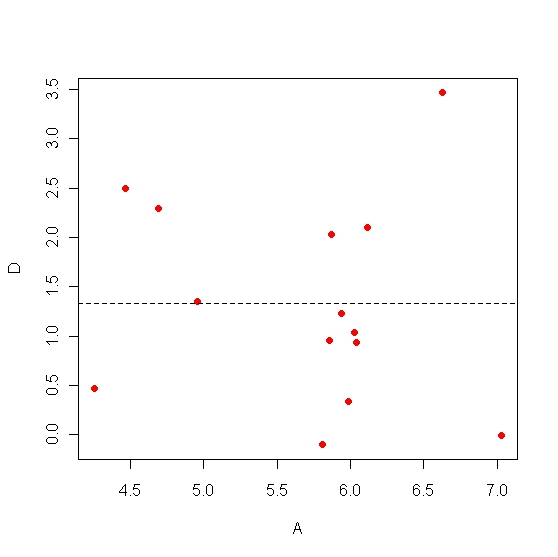
\includegraphics[scale = 0.40]{SimpleBAplot}
\end{center}
\end{frame}

\subsection{Interpreting Bland-Altman Plots}
\begin{frame}
\frametitle{Using Bland-Altman Plots}
Bland-Altman plots are a powerful graphical methodology for making
a visual assessment of the data. \alert{BA83} express the
motivation for this plot thusly:
\begin{quote}
``From this type of plot it is much easier to assess the magnitude
of disagreement (both error and bias), spot outliers, and see
whether there is any trend, for example an increase in
(difference) for high values. This way of plotting the data is a
very powerful way of displaying the results of a method comparison
study."
\end{quote}
\end{frame}
%%%%%%%%%%%%%%%%%%%%%%%%%%%%%%%%%%%%%%%%%%%%%%%%%%%%%%%%%%%%%%%%%%%%%%%%%%%%%%%%%%%%%%
\begin{frame}
\begin{itemize}
\item The Bland-Altman plot is simply a scatterplot of the case-wise
averages and differences of two methods of measurement. 
\item As the
objective of the Bland-Altman plot is to advise on the agreement
of two methods, it is the case-wise differences that are
particularly. 
\item Later it will be shown that case-wise differences
are the sole component of the next part of the methodology, the
limits of agreement.
\end{itemize}

\end{frame}
%%%%%%%%%%%%%%%%%%%%%%%%%%%%%%%%%%%%%%%%%%%%%%%%%%%%%%%%%%%%%%%%%%%%%%%%%%%%%%%%%%%%%%
\begin{frame}

\begin{itemize}
\item For creating plots, the case wise-averages fulfil several
functions, such as expressing the range over which the values were
taken, and assessing whether the assumptions of constant variance
holds.
\item Case-wise averages also allow the case-wise differences to
be presented on a two-dimensional plot, with better data
visualization qualities than a one dimensional plot.
\item \alert{BA86}
cautions that it would be the difference against either
measurement value instead of their average , as the difference
relates to both value.
\end{itemize}
\end{frame}
%%%%%%%%%%%%%%%%%%%%%%%%%%%%%%%%%%%%%%%%%%%%%%%%%%%%%%%%%%%%%%%%%%%%%%%%%%%%%%%%%%%%%%
\begin{frame}
\textbf{Next Slide}
\begin{itemize}
\item The Bland-Altman plot for comparing the `Fotobalk' and `Counter'
methods, which shall henceforth be referred to as the `F vs C'
comparison,  is depicted in Figure 1.2, using data from Table 1.3.
\item The presence and magnitude of the inter-method bias is indicated
by the dashed line.
\end{itemize}
\end{frame}
%%%%%%%%%%%%%%%%%%%%%%%%%%%%%%%%%%%%%%%%%%%%%%%%%%%%%%%%%%%%%%%%%%%%%%%%%%%%%%%%%%%%%%
\begin{frame}
\begin{figure}[h!]
\begin{center}
  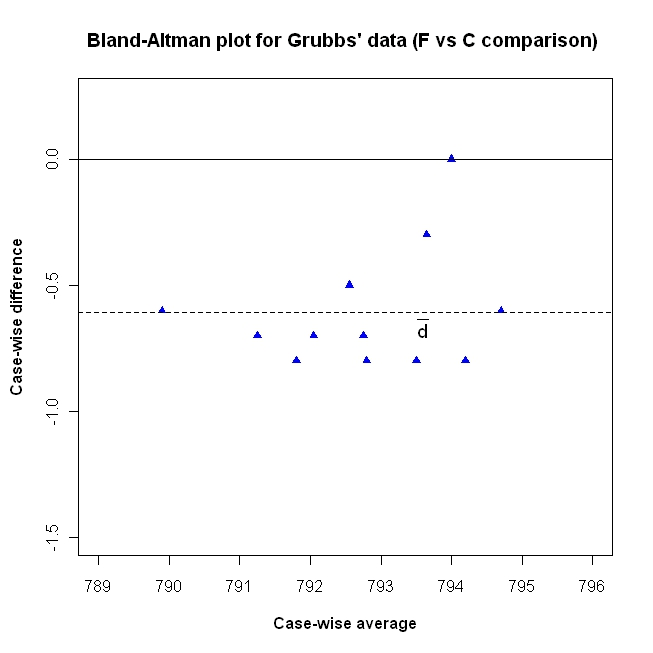
\includegraphics[width=70mm]{GrubbsBAplot-noLOA.jpeg}
  \caption{Bland-Altman plot For Fotobalk and Counter methods.}\label{GrubbsBA-noLOA}
\end{center}
\end{figure}
\end{frame}
%%%%%%%%%%%%%%%%%%%%%%%%%%%%%%%%%%%%%%%%%%%%%%%%%%%%%%%%%%%%%%%%%%%%%%%%%%%%%%%%%%%%%%
\begin{frame}
\textbf{Next Slide}

In Figure 1.3 Bland-Altman plots for the `F vs C' and `F vs T'
comparisons are shown, where `F vs T' refers to the comparison of
the `Fotobalk' and `Terma' methods. Usage of the Bland-Altman plot
can be demonstrate in the contrast between these comparisons.
\end{frame}
%%%%%%%%%%%%%%%%%%%%%%%%%%%%%%%%%%%%%%%%%%%%%%%%%%%%%%%%%%%%%%%%%%%%%%%%%%%%%%%%%%%%%%
\begin{frame}

\begin{figure}[h!]
\begin{center}
  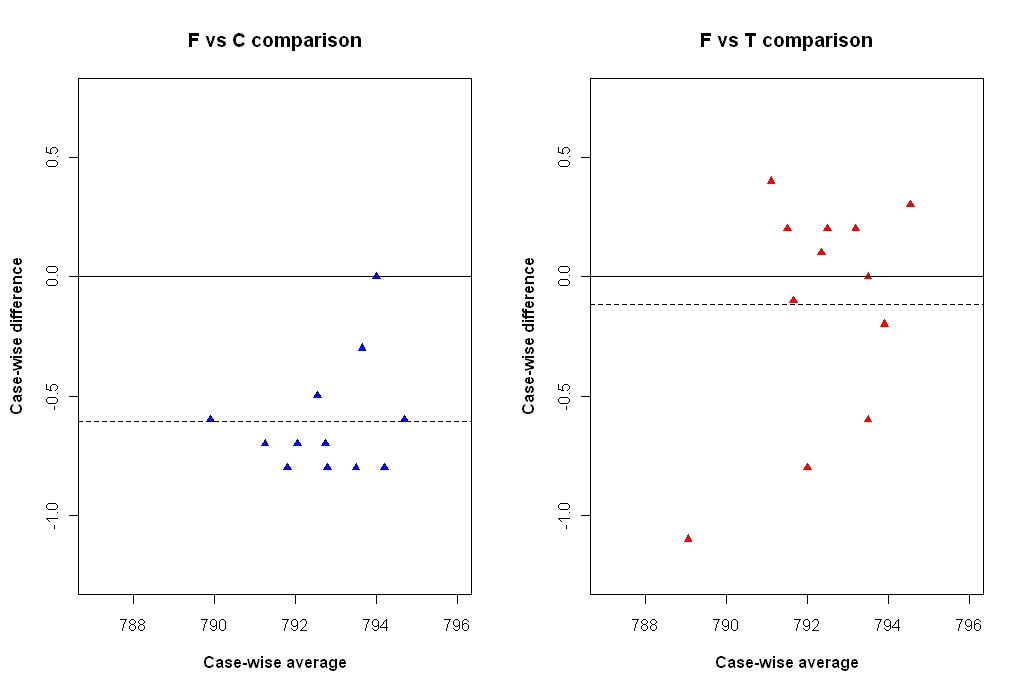
\includegraphics[height=80mm]{GrubbsDataTwoBAplots.jpeg}
  \caption{Bland-Altman plots for Grubbs' F vs C and F vs T comparisons.}\label{GrubbsDataTwoBAplots}
\end{center}
\end{figure}
\end{frame}
%%%%%%%%%%%%%%%%%%%%%%%%%%%%%%%%%%%%%%%%%%%%%%%%%%%%%%%%%%%%%%%%%%%%%%%%%%%%%%%%%%%%%%
\begin{frame}
\begin{itemize}
\item By inspection, there exists a larger inter-method bias in the `F
vs C' comparison than in the `F vs T' comparison. 
\item Conversely there
appears to be less precision in`F vs T' comparison, as indicated
by the greater dispersion of co-variates.

\item Figures 1.4, 1.5 and 1.6 are three prototype Bland-Altman plots
derived from simulated data, each for the purpose of demonstrating
how the plot would inform an analyst of features that would
adversely affect use of the recommended methodology.
\end{itemize}

\end{frame}
%------------------------------------------------------------------------%

\begin{frame}{\bf \tcb{Replicate Measurements}}
\begin{itemize}\itemsep0.7cm
\item Bland and Altman's approach originally devised for a single measurement on each item by each of the methods.
\item Their 1999 paper \cite{BA99} extended their approach to replicate measurements:\\ \emph{By replicates we mean two or more measurements on the same
individual taken in identical conditions. \\In general this requirement means that the
measurements are taken in quick succession. }
\item Emphasis put on "repeatability".
\end{itemize}
\end{frame}

%%%%%%%%%%%%%%%%%%%%%%%%%%%%%%%%%%%%%%%%%%%%%%%%%%%%%%%%%%%%%%%%%%%%%%%%%%%%%%%%%%%%%%
%\begin{frame}
%Figure 1.4 demonstrates how the Bland-Altman plot would indicate
%increasing variance of differences over the measurement range.
%Fitted regression lines, for both the upper and lower half of the
%plot, has been added to indicate the trend. Figure 1.5 is an
%example of cases where the inter-method bias changes over the
%measurement range. This is known as proportional bias. In both
%Figures 1.4 and 1.5, the assumptions necessary for further
%analysis using the limits of agreement are violated.
%\end{frame}

%%%%%%%%%%%%%%%%%%%%%%%%%%%%%%%%%%%%%%%%%%%%%%%%%%%%%%%%%%%%%%%%%%%%%%%%%%%%%%%%%%%%%%
\begin{frame}
\begin{figure}[h!]
\begin{center}
  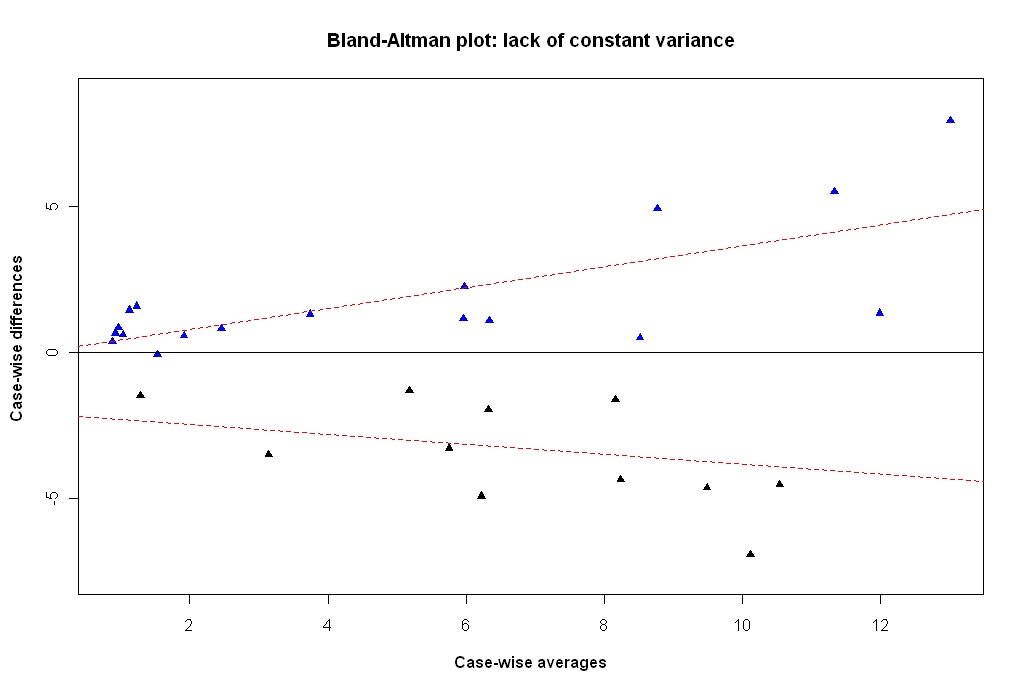
\includegraphics[height=90mm]{BAFanEffect.jpeg}
  \caption{Bland-Altman plot demonstrating the increase of variance over the range.}\label{BAFanEffect}
\end{center}
\end{figure}

\begin{figure}[h!]
\begin{center}
  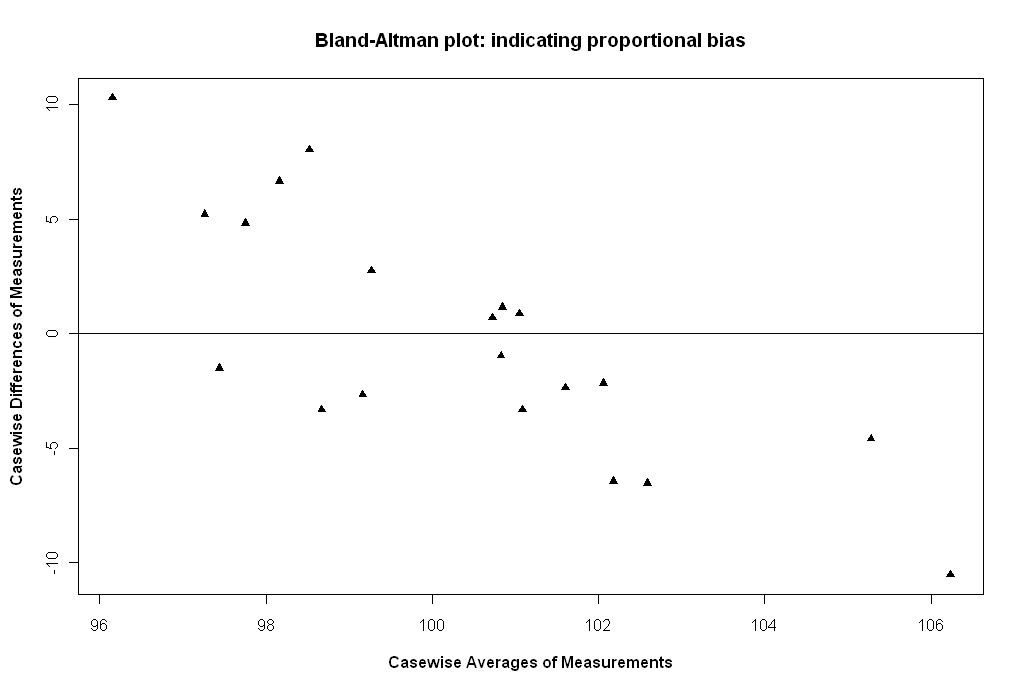
\includegraphics[height=90mm]{PropBias.jpeg}
  \caption{Bland-Altman plot indicating the presence of proportional bias.}\label{PropBias}
\end{center}
\end{figure}
\end{frame}
%%%%%%%%%%%%%%%%%%%%%%%%%%%%%%%%%%%%%%%%%%%%%%%%%%%%%%%%%%%%%%%%%%%%%%%%%%%%%%%%%%%%%%
\begin{frame}
\begin{figure}[h!]
\begin{center}
  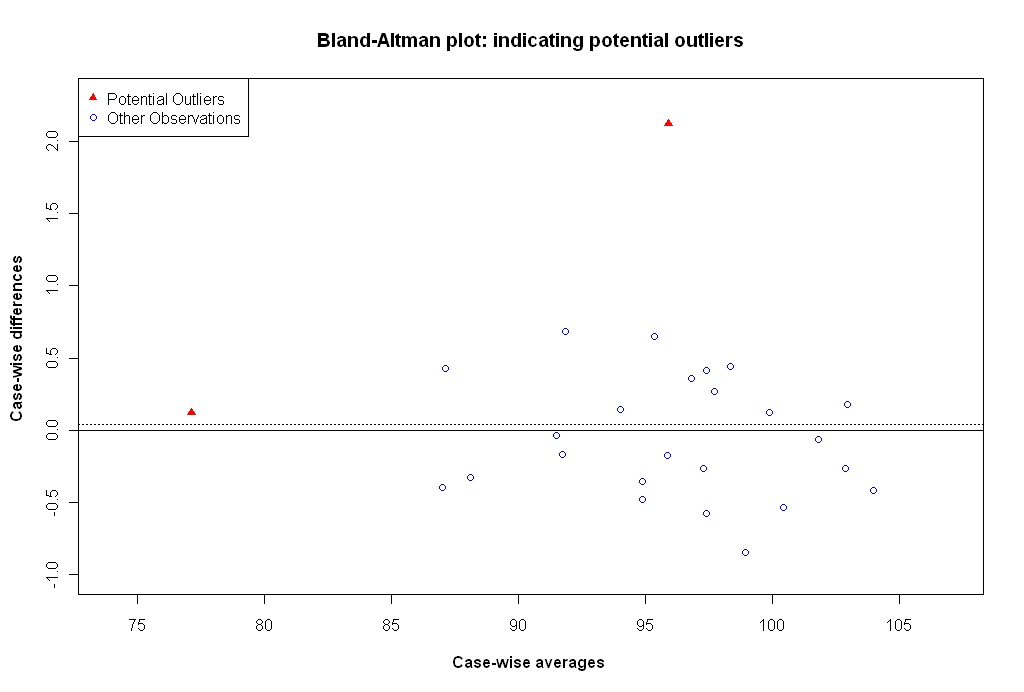
\includegraphics[width=125mm]{BAOutliers.jpeg}
  \caption{Bland-Altman plot indicating the presence of potential outliers.}\label{Outliers}
\end{center}
\end{figure}

\end{frame}
%%%%%%%%%%%%%%%%%%%%%%%%%%%%%%%%%%%%%%%%%%%%%%%%%%%%%%%%%%%%%%%%%%%%%%%%%%%%%%%%%%%%%%
\subsection{Replicate Measurements}
\begin{frame}


Thus far, the formulation for comparison of two measurement
methods is one where one measurement by each method is taken on
each subject. Should there be two or more measurements by each
methods, these measurement are known as `replicate measurements'.
\alert{BXC2008} recommends the use of replicate measurements, but
acknowledges that  additional computational complexity.
\end{frame}

%%%%%%%%%%%%%%%%%%%%%%%%%%%%%%%%%%%%%%%%%%%%%%%%%%%%%%%%%%%%%%%%%%%%%%%%%%%%%%%%%%%%%%
\begin{frame}
\alert{BA86} address this problem by offering two different
approaches. The premise of the first approach is that replicate
measurements can be treated as independent measurements. The
second approach is based upon using the mean of the each group of
replicates as a representative value of that group. Using either
of these approaches will allow an analyst to estimate the inter
method bias.

%\subsubsection{Mean of Replicates Limits of Agreement}

However, because of the removal of the effects of the replicate
measurements error, this would cause the estimation of the
standard deviation of the differences to be unduly small.
\alert{BA86} propose a correction for this.
\end{frame}
%%%%%%%%%%%%%%%%%%%%%%%%%%%%%%%%%%%%%%%%%%%%%%%%%%%%%%%%%%%%%%%%%%%%%%%%%%%%%%%%%%%%%%
\begin{frame}
\alert{BXC2008} takes issue with the limits of agreement based on
mean values, in that they can only be interpreted as prediction
limits for difference between means of repeated measurements by
both methods, as opposed to the difference of all measurements.
Incorrect conclusions would be caused by such a misinterpretation.
\alert{BXC2008} demonstrates how the limits of agreement
calculated using the mean of replicates are `much too narrow as
prediction limits for differences between future single
measurements'. This paper also comments that, while treating the
replicate measurements as independent will cause a downward bias
on the limits of agreement calculation, this method is preferable
to the `mean of replicates' approach.
\end{frame}
%--------------------------------------------------------------------- %


%----------------------------------------------------------- %
\section{Regression Methods - "mcr" and Deming regression}

\begin{frame}
\frametitle{REgression Techniques for MCS}
\textbf{Regression Based Techniques}
\end{frame}

\begin{frame}
\begin{itemize}
\item Conventional regression models are estimated using the ordinary
least squares (OLS) technique, and are referred to as `Model I
regression'\alert{CornCoch,ludbrook97}. 
\item A key feature of Model I
models is that the independent variable is assumed to be measured
without error. As often pointed out in several papers
\alert{BA83,ludbrook97}, this assumption invalidates simple linear
regression for use in method comparison studies, as both methods
must be assumed to be measured with error.
\end{itemize}

\end{frame}
%%%%%%%%%%%%%%%%%%%%%%%%%%%%%%%%%%%%%%%%%%%%%%%%%%%%%%%%%%%%%%%%%%%%%%%%%%%%%%%%%%%%%%
\begin{frame}
\begin{itemize}
\item
The use of regression models that assumes the presence of error in
both variables $X$ and $Y$ have been proposed for use instead.
\alert{CornCoch,ludbrook97}, These methodologies are collectively
known as `Model II regression'. They differ in the method used to
estimate the parameters of the regression.

\item Regression estimates depend on formulation of the model. A
formulation with one method considered as the $X$ variable will
yield different estimates for a formulation where it is the $Y$
variable. 
\item With Model I regression,the models fitted in both cases
will entirely different and inconsistent. However with Model II
regression, they will be consistent and complementary.
\end{itemize}

\end{frame}

%%%%%%%%%%%%%%%%%%%%%%%%%%%%%%%%%%%%%%%%%%%%%%%%%%%%%%%%%%%%%%%%%%%%%%%%%%%%%%%%%%%%%%

%---------------------------------------------------------- %
\subsection{Error in Variables Deming Regression}
\begin{frame}


\textbf{Deming Regression}
\begin{itemize}
\item Both Variables are assumed to have attended measurement error.
\item Orthonormal Regression (Variance Ratio's are assumed to be equal)
\item Deming Regression (Variance Ration is specifed, with default setting of 1)
\item Dunn 2002 advises caution with model
\item Model Diagnostics?
\end{itemize}

\end{frame}
%%%%%%%%%%%%%%%%%%%%%%%%%%%%%%%%%%%%%%%%%%%%%%%%%%%%%%%%%%%%%%%%%%%%%%%%%%%%%%%%%%%%%%
\begin{frame}
\textbf{Editing Comments}
\begin{itemize}
\item
\item
\item
\item 
\end{itemize}
\end{frame}
\subsection{Deming's Regression}
\begin{frame}

\begin{itemize}
\item The most commonly known Model II methodology is known as Deming's
Regression, (also known an Ordinary Least Product regression).
Deming regression is recommended by \alert{CornCoch} as the
preferred Model II regression for use in method comparison
studies. 
\item As previously noted, the Bland Altman Plot is
uninformative about the comparative influence of proportional bias
and fixed bias. Deming's regression provides independent tests for
both types of bias.

\item For a given $\lambda$, \alert{Kummel} derived the following
estimate for the Demimg regression slope parameter. ($\alpha$ is
simply estimated by using the identity
$\bar{Y}-\hat{\beta}\bar{X}$.)
\begin{equation}
\hat{\beta} =\quad \frac{S_{YY} - \lambda S_{XX}+[(S_{YY} -
\lambda S_{XX})^{2}+ 4\lambda S^{2}_{XY}]^{1/2}}{2S_{XY}}
\end{equation}
\end{itemize}
\end{frame}
%%%%%%%%%%%%%%%%%%%%%%%%%%%%%%%%%%%%%%%%%%%%%%%%%%%%%%%%%%%%%%%%%%%%%%%%%%%%%%%%%%%%%%
\begin{frame}
\frametitle{Deming Regression}
As with conventional regression methodologies, Deming's regression
calculates an estimate for both the slope and intercept for the
fitted line, and standard errors thereof. Therefore there is
sufficient information to carry out hypothesis tests on both
estimates, that are informative about presence of fixed and
proportional bias.
\end{frame}
%%%%%%%%%%%%%%%%%%%%%%%%%%%%%%%%%%%%%%%%%%%%%%%%%%%%%%%%%%%%%%%%%%%%%%%%%%%%%%%%%%%%%%
\begin{frame}
\frametitle{Deming Regression}
A $95\%$ confidence interval for the intercept estimate can be
used to test the intercept, and hence fixed bias, is equal to
zero. This hypothesis is accepted if the confidence interval for
the estimate contains the value $0$ in its range. Should this be,
it can be concluded that fixed bias is not present. Conversely, if
the hypothesis is rejected, then it is concluded that the
intercept is non zero, and that fixed bias is present.
\end{frame}
%%%%%%%%%%%%%%%%%%%%%%%%%%%%%%%%%%%%%%%%%%%%%%%%%%%%%%%%%%%%%%%%%%%%%%%%%%%%%%%%%%%%%%
\begin{frame}
Testing for proportional bias is a very similar procedure. The
$95\%$ confidence interval for the slope estimate can be used to
test the hypothesis that the slope is equal to $1$. This
hypothesis is accepted if the confidence interval for the estimate
contains the value $1$ in its range. If the hypothesis is
rejected, then it is concluded that the slope is significant
different from $1$ and that a proportional bias exists.
\end{frame}


%%%%%%%%%%%%%%%%%%%%%%%%%%%%%%%%%%%%%%%%%%%%%%%%%%%%%%%%%%%%%%%%%%%%%%%%%%%%%%%%%%%%%%
\begin{frame}
For convenience, a new data set shall be introduced to demonstrate
Demings regression. Measurements of transmitral volumetric flow
(MF) by doppler echocardiography, and left ventricular stroke
volume (SV) by cross sectional echocardiography in 21 patients
withour aortic valve disease are tabulated in \alert{zhang}. This
data set features in the discussion of method comparison studies
in \alert[p.398]{AltmanBook} .

\end{frame}
%%%%%%%%%%%%%%%%%%%%%%%%%%%%%%%%%%%%%%%%%%%%%%%%%%%%%%%%%%%%%%%%%%%%%%%%%%%%%%%%%%%%%%
\begin{frame}

% latex table generated in R 2.6.0 by xtable 1.5-5 package
% Tue Sep 01 13:31:17 2009
\begin{table}[h!]
\begin{center}
\begin{tabular}{|c|c|c||c|c|c||c|c|c|}
  \hline
 Patient & MF  & SV  & Patient & MF  & SV  & Patient & MF  & SV \\
 &($cm^{3}$)&  ($cm^{3}$) & &($cm^{3}$)&  ($cm^{3}$) & &($cm^{3}$)&  ($cm^{3}$)
 \\
  \hline
1 & 47 & 43 &  8 & 75 & 72 &  15 & 90 & 82 \\
  2 & 66 & 70 & 9 & 79 & 92 &  16 & 100 & 100 \\
  3 & 68 & 72 & 10 & 81 & 76 & 17 & 104 & 94 \\
  4 & 69 & 81 & 11 & 85 & 85 &  18 & 105 & 98 \\
  5 & 70 & 60 & 12 & 87 & 82 & 19 & 112 & 108 \\
  6 & 70 & 67 & 13 & 87 & 90 & 20 & 120 & 131 \\
  7 & 73 & 72 & 14 & 87 & 96 &  21 & 132 & 131 \\

   \hline
\end{tabular}
\caption{Transmitral volumetric flow(MF) and left ventricular
stroke volume (SV) in 21 patients. (Zhang et al 1986)}
\end{center}
\end{table}
\newpage
%\begin{figure}[h!]
%  % Requires \usepackage{graphicx}
%  \includegraphics[width=130mm]{ZhangDeming.jpeg}
%  \caption{Deming Regression For Zhang's Data}\label{ZhangDeming}
%\end{figure}

\end{frame}
%%%%%%%%%%%%%%%%%%%%%%%%%%%%%%%%%%%%%%%%%%%%%%%%%%%%%%%%%%%%%%%%%%%%%%%%%%%%%%%%%%%%%%
\begin{frame}
\frametitle{Deming Regression}
Deming's Regression suffers from some crucial drawback. Firstly it
is computationally complex, and it requires specific software
packages to perform calculations.Secondly it is uninformative
about the comparative precision of two methods of measurement.
Most importantly \alert{CarollRupert} states that Deming's
regression is acceptable only when the precision ratio ($\lambda$,
in their paper as $\eta$) is correctly specified ,but in practice
this is often not the case, with the $\lambda$ being
underestimated.
\end{frame}
%%%%%%%%%%%%%%%%%%%%%%%%%%%%%%%%%%%%%%%%%%%%%%%%%%%%%%%%%%%%%%%%%%%%%%%%%%%%%%%%%%%%%%

%------------------------------------------------------------%
\section{Unscaled Indices - Using TDI and CP}
\begin{frame}
\frametitle{Using TDI and CP}
\begin{itemize}
\item Total Deviation Index
\item Coverage Probability
\item Mountain Plots (Krouwer and Monti)
\end{itemize}

\end{frame}
%\chapter{Linear Mixed Effects Models}
%------------------------------------------------------------%
\section{LME models in Method comparison}

\begin{frame}
\frametitle{Using LME Models}
\textbf{Section 7 - Using LME Models in Method comparison}
\begin{itemize}
\item Carstensen et al 
\item Roy 2009
\end{itemize}
\end{frame}


%With the greater computing power available for scientific
%analysis, it is inevitable that complex models such as linear
%mixed effects models should be applied to method comparison
%studies.







% \begin{equation}
% data here
% \end{equation}



%%%%%%%%%%%%%%%%%%%%%%%%%%%%%%%%%%%%%%%%%%%%%%%%%%%%%%%%%%%%%%%%%%%%%%%%%%%%%%%%%%%%%%

\begin{frame}
\alert{BXC2008} sets out a methodology of computing the limits of
agreement based upon variance component estimates derived using
linear mixed effects models. Measures of repeatability, a
characteristic of individual methods of measurements, are also
derived using this method.
\end{frame}
%%%%%%%%%%%%%%%%%%%%%%%%%%%%%%%%%%%%%%%%%%%%%%%%%%%%%%%%%%%%%%%%%%%%%%%%%%%%%%%%%%%%%%
\subsection{Using LME models to create Prediction Intervals}

\begin{frame}
\alert{BXC2004} also advocates the use of linear mixed models in
the study of method comparisons. The model is constructed to
describe the relationship between a value of measurement and its
real value. 

The non-replicate case is considered first, as it is
the context of the Bland-Altman plots. This model assumes that
inter-method bias is the only difference between the two methods.
A measurement $y_{mi}$ by method $m$ on individual $i$ is
formulated as follows;
\begin{equation}
y_{mi}  = \alpha_{m} + \mu_{i} + e_{mi} \qquad ( e_{mi} \sim
N(0,\sigma^{2}_{m}))
\end{equation}
\end{frame}
%%%%%%%%%%%%%%%%%%%%%%%%%%%%%%%%%%%%%%%%%%%%%%%%%%%%%%%%%%%%%%%%%%%%%%%%%%%%%%%%%%%%%%
\begin{frame}
The differences are expressed as $d_{i} = y_{1i} - y_{2i}$ For the
replicate case, an interaction term $c$ is added to the model,
with an associated variance component. All the random effects are
assumed independent, and that all replicate measurements are
assumed to be exchangeable within each method.

\begin{equation}
y_{mir}  = \alpha_{m} + \mu_{i} + c_{mi} + e_{mir} \qquad ( e_{mi}
\sim N(0,\sigma^{2}_{m}), c_{mi} \sim N(0,\tau^{2}_{m}))
\end{equation}
%%%%%%%%%%%%%%%%%%%%%%%%%%%%%%%%%%%%%%%%%%%%%%%%%%%%%%%%%%%%%%%%%%%%%%%%%%%%%%%%%%%%%%

\end{frame}
%%%%%%%%%%%%%%%%%%%%%%%%%%%%%%%%%%%%%%%%%%%%%%%%%%%%%%%%%%%%%%%%%%%%%%%%%%%%%%%%%%%%%%
%------------------------------------------------------------%
\subsection[Carstensen's Mixed Models]{Carstensen's Mixed Models}

\Large

%----------------------------------------------------------- %
 %SLIDE 1

\begin{frame}{\bf \tcb{Carstensen's Mixed Models}}
\begin{itemize}
\item Carstensen \textit{et al} \cite{BXC2004} proposes linear mixed effects models for deriving
conversion calculations similar to Deming's regression, and for
estimating variance components for measurements by different
methods. 
%\item The following model (in the authors own notation) is
%formulated as follows, where $y_{mir}$ is the $r$th replicate
%measurement on subject $i$ with method $m$.
\end{itemize}
\end{frame}
%---------------------------------------------------------- %
 %SLIDE 2
\begin{frame}

\begin{itemize}
\item The following model (in the authors own notation) is
formulated as follows, where $y_{mir}$ is the $r$th replicate
measurement on subject $i$ with method $m$.
\end{itemize}
{
\LARGE
\begin{equation}
y_{mir}  = \alpha_{m} + \beta_{m}\mu_{i} + c_{mi} + e_{mir} 
\end{equation}
}
\vspace{0.3cm}
{
\normalsize
\[ e_{mi} \sim N(0,\sigma^{2}_{m}), c_{mi} \sim N(0,\tau^{2}_{m})\]
}
\end{frame}
%------------------------------------------------------- %
 %SLIDE 3
\begin{frame}[fragile]
\frametitle{Carstensen's Mixed Models}
\begin{itemize}
\item The intercept term $\alpha$ and the $\beta_{m}\mu_{i}$ term follow
from \textit{Dunn} \cite{DunnSEME}, expressing constant and proportional bias
respectively , in the presence of a real value $\mu_{i}.$
\item $c_{mi}$ is a interaction term to account for replicate, and
 $e_{mir}$ is the residual associated with each observation.
\item Since variances are specific to each method, this model can be
fitted separately for each method.
\end{itemize}

\end{frame}
%---------------------------------------------------------------- %
\begin{frame}
\frametitle{Carstensen's Mixed Models}
\begin{itemize}
\item The above formulation doesn't require the data set to be balanced.
However, it does require a sufficient large number of replicates
and measurements to overcome the problem of identifiability. 
\item The
import of which is that more than two methods of measurement may
be required to carry out the analysis. 
\end{itemize}

\end{frame}
%---------------------------------------------------------------- %
\begin{frame}
\frametitle{Carstensen's Mixed Models}
\begin{itemize}
\item There is also the
assumptions that observations of measurements by particular
methods are exchangeable within subjects. \item \textbf{\textit{Exchangeability}} means
that future samples from a population behaves like earlier
samples).
\end{itemize}
\end{frame}
%---------------------------------------------------------------- %

%-----------------------%
\begin{frame}
\frametitle{Computing LoAs from LME models}
\emph{
One important feature of replicate observations is that they should be independent
of each other. In essence, this is achieved by ensuring that the observer makes each
measurement independent of knowledge of the previous value(s). This may be difficult
to achieve in practice.}
\end{frame}

\subsection*{Using LME models to create Prediction Intervals}

\begin{frame}
\Large
\begin{itemize}
\item Carstensen \textit{et al} \cite{BXC2004} also advocates the use of linear mixed models in
the study of method comparisons. The model is constructed to
describe the relationship between a value of measurement and its
real value.
\item  The non-replicate case is considered first, as it is
the context of the Bland Altman plots. This model assumes that
inter-method bias is the only difference between the two methods.
A measurement $y_{mi}$ by method $m$ on individual $i$ is
formulated as follows;
\end{itemize}
\begin{equation}
y_{mi}  = \alpha_{m} + \mu_{i} + e_{mi} \qquad ( e_{mi} \sim
N(0,\sigma^{2}_{m}))
\end{equation}

\end{frame}
\begin{frame}
\Large
\begin{itemize}
\item The differences are expressed as $d_{i} = y_{1i} - y_{2i}$ For the
replicate case, an interaction term $c$ is added to the model,
with an associated variance component. 
\item All the random effects are
assumed independent, and that all replicate measurements are
assumed to be exchangeable within each method.
\end{itemize}
\begin{eqnarray}
y_{mir}  = \alpha_{m} + \mu_{i} + c_{mi} + e_{mir} 
\end{eqnarray}

%\[  e_{mi} \sim N(0,\sigma^{2}_{m}) \c_{mi} \sim N(0,\tau^{2}_{m}) \]
%\end{eqnarray}
\end{frame}

\begin{frame}
\Large
\begin{itemize}
\item Carstensen \textit{et al} \cite{BXC2008} proposes a methodology to calculate prediction
intervals in the presence of replicate measurements, overcoming
problems associated with Bland-Altman methodology in this regard.
\item It is not possible to estimate the interaction variance components
$\tau^{2}_{1}$ and $\tau^{2}_{2}$ separately. Therefore it must be
assumed that they are equal. The variance of the difference can be
estimated as follows:
\begin{equation}
var(y_{1j}-y_{2j})
\end{equation}
\end{itemize}
\end{frame}

\section{Computing LoAs from LME models}
%--------------------------%

\begin{frame}
\textbf{Section 8 computing LoAs from LME models}

\begin{itemize}
\item
\end{itemize}
\end{frame}
%--------------------------%

\begin{frame}
\emph{
One important feature of replicate observations is that they should be independent
of each other. In essence, this is achieved by ensuring that the observer makes each
measurement independent of knowledge of the previous value(s). This may be difficult
to achieve in practice.}
\end{frame}


%-------------------------------------------------------------------------------------%
\begin{frame}
\frametitle{Roy's method}
\begin{itemize}
\item Roy proposes a novel method using the LME model with Kronecker product covariance structure in a doubly multivariate set-up to assess the agreement between a new method and an established method with unbalanced data and with unequal replications for different subjects (alert{Roy}).
\item 
Using Roy's method, four candidate models are constructed, each differing by constraints applied to the variance covariance matrices.
\item In addition to computing the inter-method bias, three significance tests are carried out on the respective formulations to make a judgement on whether or not two methods are in agreement.
\end{itemize}
\end{frame}

%---------------------------------------------%
\begin{frame}
\frametitle{Method Comparison Studies with \texttt{R}}
\large
\begin{itemize}
\item 
The absence of inter-method bias by itself is not sufficient to
establish whether two measurement methods agree. 
\item The two
methods must also have equivalent levels of precision. 
\item Should one
method yield results considerably more variable than that of the
other, they can not be considered to be in agreement. 
\item With this in
mind a methodology is required that allows an analyst to estimate
the inter-method bias, and to compare the precision of both
methods of measurement.
\end{itemize}
\end{frame}

\subsection{Carstensen's Mixed Models}
\begin{frame}
\alert{BXC2004} proposes linear mixed effects models for deriving
conversion calculations similar to Deming's regression, and for
estimating variance components for measurements by different
methods. The following model ( in the authors own notation) is
formulated as follows, where $y_{mir}$ is the $r$th replicate
measurement on subject $i$ with method $m$.

\begin{equation}
y_{mir}  = \alpha_{m} + \beta_{m}\mu_{i} + c_{mi} + e_{mir} \qquad
( e_{mi} \sim N(0,\sigma^{2}_{m}), c_{mi} \sim N(0,\tau^{2}_{m}))
\end{equation}
\end{frame}
%%%%%%%%%%%%%%%%%%%%%%%%%%%%%%%%%%%%%%%%%%%%%%%%%%%%%%%%%%%%%%%%%%%%%%%%%%%%%%%%%%%%%%
\begin{frame}
The intercept term $\alpha$ and the $\beta_{m}\mu_{i}$ term follow
from \alert{DunnSEME}, expressing constant and proportional bias
respectively , in the presence of a real value $\mu_{i}.$
 $c_{mi}$ is a interaction term to account for replicate, and
 $e_{mir}$ is the residual associated with each observation.
Since variances are specific to each method, this model can be
fitted separately for each method.
\end{frame}
%%%%%%%%%%%%%%%%%%%%%%%%%%%%%%%%%%%%%%%%%%%%%%%%%%%%%%%%%%%%%%%%%%%%%%%%%%%%%%%%%%%%%%
\begin{frame}
\begin{itemize}
\item The above formulation doesn't require the data set to be balanced.
However, it does require a sufficient large number of replicates
and measurements to overcome the problem of identifiability. The
import of which is that more than two methods of measurement may
be required to carry out the analysis. 
\item There is also the
assumptions that observations of measurements by particular
methods are exchangeable within subjects. (Exchangeability means
that future samples from a population behaves like earlier
samples).
\end{itemize}


%\alert{BXC2004} describes the above model as a `functional model',
%similar to models described by \alert{Kimura}, but without any
%assumptions on variance ratios. A functional model is . An
%alternative to functional models is structural modelling
\end{frame}
%%%%%%%%%%%%%%%%%%%%%%%%%%%%%%%%%%%%%%%%%%%%%%%%%%%%%%%%%%%%%%%%%%%%%%%%%%%%%%%%%%%%%%
\begin{frame}
\alert{BXC2004} uses the above formula to predict observations for
a specific individual $i$ by method $m$;

\begin{equation}BLUP_{mir} = \hat{\alpha_{m}} + \hat{\beta_{m}}\mu_{i} +
c_{mi} \end{equation}. Under the assumption that the $\mu$s are
the true item values, this would be sufficient to estimate
parameters. When that assumption doesn't hold, regression
techniques (known as updating techniques) can be used additionally
to determine the estimates. The assumption of exchangeability can
be unrealistic in certain situations. \alert{BXC2004} provides an
amended formulation which includes an extra interaction term ($
d_{mr} \sim N(0,\omega^{2}_{m}$)to account for this.

\end{frame}


%------------------------------------------------------------%
\subsection{Roy's Hypothesis Tests for MCS}


% Use London R stuff here
\begin{frame}
\frametitle{Editing Notes - Roys 2009 paper}
\begin{itemize}
\item 
\item
\end{itemize}
\end{frame}
\subsection*{Roy's LME Model}
%------------------------------------------------------------------------%
\begin{frame}{\bf \tcb{LME models}}
\begin{itemize}\itemsep0.7cm
\item In a linear mixed-effects model, responses from a subject are due to both fixed and random
effects. A random effect is an effect associated with a sampling procedure.
\item Replicate measurements would require use of random effect terms in model.
\item Can have differing number of replicate measurements for different subjects.
\end{itemize}
\end{frame}


%--------------------------------------------------------------------------------------------------------%
%Include a Short Section on Hamlett in the notes - for reading after the talk

\begin{frame}
\frametitle{Hmalett}
\large

\begin{itemize}
\item Hamlett re-analyses the data of \textbf{Lam} to generalize their model to cover other settings not covered by the Lam method.

\item In many cases, repeated observation are collected from each subject in sequence  and/or longitudinally.


\[ y_i = \alpha + \mu_i + \epsilon \]
\end{itemize}

\end{frame}
%--------------------------------------------------------------------------------------------------------%


\begin{frame}
\frametitle{Hmalett}
The classical model is based on measurements $y_{mi}$
by method $m=1,2$ on item $i = 1,2 \ldots$

\[y_{mi} + \alpha_{m} + \mu_{i} + e_{mi}\]

\[e_{mi} \sim \mathcal{n} (0,\sigma^2_m)\]

Even though the separate variances can not be
identified, their sum can be estimated by the empirical variance of the differences.

Like wise the separate $\alpha$ can not be
estimated, only theiir difference can be estimated as
$\bar{D}$

\end{frame}
%------------------------------------------------------------------------%
\begin{frame}{\bf \tcb{Roy's Approach}}
\begin{itemize}\itemsep0.7cm
\item Roy proposes an LME model with Kronecker product covariance structure in a doubly multivariate setup.
\item Response for $i$th subject can be written as
\[ y_i = \beta_0 + \beta_1x_{i1} + \beta_2x_{i2} + b_{1i}z_{i1}  + b_{2i}z_{i2} + \epsilon_i \]
\item $\beta_1$ and $\beta_2$ are fixed effects corresponding to both methods. ($\beta_0$ is the intercept.)
\item $b_{1i}$ and $b_{2i}$ are random effects corresponding to both methods.
\end{itemize}
\end{frame}

%------------------------------------------------------------------------%
\begin{frame}{\bf \tcb{Roy's LME model}}
\begin{itemize}\itemsep0.7cm

\item Let $\boldsymbol{y}_i$ be the set of responses for subject $i$ ( in matrix form).
\item $\boldsymbol{y}_i = \boldsymbol{X}_i\boldsymbol{\beta} + \boldsymbol{Z}_i \boldsymbol{b}_i + \boldsymbol{\epsilon}_i$
\item $\boldsymbol{b}_i \sim N_m(0,\boldsymbol{D})$  (m: number of methods)
\item $\boldsymbol{\epsilon}_i \sim N_{n_i}(0,\boldsymbol{R})$ ($n_i$: number of measurements on subject $i$)
\end{itemize}
\end{frame}

%------------------------------------------------------------------------%


\begin{frame}{\bf \tcb{Variance-covariance matrix}}
\begin{itemize}
\item Overall variance covariance matrix for response vector $\boldsymbol{y}_i$

\[ \mbox{Cov}(\boldsymbol{y}_i)= \boldsymbol{Z}_i \boldsymbol{D}\boldsymbol{Z}^{\prime}_i + \boldsymbol{R}_i \]

\item can be re-expressed as follows:
\[\boldsymbol{Z}_i \left[ \begin{array}{cc} d^2_1 & d_{12}\\
d_{12} & d^2_2\\ \end{array}\right]\boldsymbol{Z}^{\prime}_i  +  \left(V \otimes \left[\begin{array}{cc} \sigma^2_1 & \sigma_{12}\\
\sigma_{12} & \sigma^2_2\\ \end{array}\right] \right)
\]

\item Overall variability between the two methods is sum of between-subject and within-subject variability,
\[
 \mbox{Block } \boldsymbol{\Omega}_i = \left[ \begin{array}{cc} d^2_1 & d_{12}\\ d_{12} & d^2_2\\ \end{array} \right]
+ \left[\begin{array}{cc} \sigma^2_1 & \sigma_{12}\\ \sigma_{12} & \sigma^2_2\\ \end{array}\right].
\]

\end{itemize}
\end{frame}


%------------------------------------------------------------------------------------------------------%
\begin{frame}
\frametitle{Roy's method}formulates a very powerful method of assessing whether two methods of measurement, with replicate measurements, also using LME models. Roy's approach is based on the construction of variance-covariance matrices.
Importantly, Roy's approach does not address the issue of limits of agreement (though another related analysis , the coefficient of repeatability, is mentioned).

\end{frame}

%------------------------------------------------------------------------------------------------------%
\begin{frame}
\frametitle{Roy's method}
This paper seeks to use Roy's approach to estimate the limits of agreement. These estimates will be compared to estimates computed under Carstensen's formulation.

In computing limits of agreement, it is first necessary to have an estimate for the standard deviations of the differences. When the agreement of two methods is analyzed using LME models, a clear method of how to compute the standard deviation is required. As the estimate for inter-method bias and the quantile would be the same for both methodologies, the focus is solely on the standard deviation.

\end{frame}

%------------------------------------------------------------------------------------------------------%
\begin{frame}
\frametitle{Roy's method}

Roy proposes a novel method using the LME model with Kronecker product covariance structure in a doubly multivariate set-up to assess the agreement between a new method and an established method with unbalanced data and with unequal replications for different subjects \alert{Roy}.

Using Roy's method, four candidate models are constructed, each differing by constraints applied to the variance covariance matrices. In addition to computing the inter-method bias, three significance tests are carried out on the respective formulations to make a judgement on whether or not two methods are in agreement.

\end{frame}
%--------------------------------------------------------------------------------------------------------------%


\section*[Implementation with \texttt{R} ]{Implementation}
\subsection{Implementation}

\begin{frame}{\bf \tcb{Variance-Covariance Structures}}
\[\left(
\begin{array}{cc}
\sigma^2_1 & \sigma_{12}\\
\sigma_{12} & \sigma^2_2\\
\end{array} \right)
\]

\begin{itemize}
\item Symmetric structure specifies that $\sigma^2_1$ may differ from $\sigma^2_2$.
\item Compound symmetric structure specifies that $\sigma^2_1 = \sigma^2_2$.
\item In both cases, $\sigma_{12}$ may take value other than 0.
\end{itemize}

\end{frame}
%------------------------------------------------------------------------%
\begin{frame}{\bf \tcb{The \texttt{nlme} Package}}

\begin{itemize}
\item LME models can be implemented in \texttt{R} using the \texttt{nlme} package, one of the core packages.\\
\item Authors: Jose Pinheiro, Douglas Bates (up to 2007), Saikat
DebRoy (up to 2002), Deepayan Sarkar (up to 2005), the \texttt{R} Core team \\(source: \texttt{nlme} package manual)\\
\item ``Mixed-Effects Models in S and S-PLUS" by JC Pinheiro and DM Bates (Springer,2000)

\end{itemize}

\end{frame}
%------------------------------------------------------------------------%
\begin{frame}[fragile]{\bf \tcb{The Reference Model}}
\texttt{REF = lme(y $\sim$ meth,\\
   \hspace{0.6cm} data = dat,\\
   \hspace{0.6cm} random = list(item=\tcr{pdSymm}($\sim$ meth-1)), \\
   \hspace{0.6cm} weights=varIdent(form=$\sim$1|meth),\\
   \hspace{0.6cm} correlation = \tcr{corSymm}(form=$\sim$1 | item/repl),\\
   \hspace{0.6cm} method="ML")}\\
\begin{itemize}
\item LME model that specifies a symmetric matrix structure for both between-subject and within-subject variances.
\end{itemize}

\end{frame}

%------------------------------------------------------------------------%
\begin{frame}[fragile]{\bf \tcb{The Nested Model 1}}
\texttt{NMB = lme(y $\sim$ meth,\\
   \hspace{0.6cm} data = dat,\\
   \hspace{0.6cm} random = list(item=\tcr{pdCompSymm}($\sim$ meth-1)), \\
   \hspace{0.6cm} weights=varIdent(form=$\sim$1|meth),\\
   \hspace{0.6cm} correlation = \tcr{corSymm}(form=$\sim$1 | item/repl),\\
   \hspace{0.6cm} method="ML")}

\begin{itemize}
\item LME model that specifies a compound symmetric matrix structure for between-subject and symmetric structure within-subject variances.
\end{itemize}

\end{frame}
%------------------------------------------------------------------------%
\begin{frame}[fragile]{\bf \tcb{The Nested Model 2}}
\texttt{NMW = lme(y $\sim$ meth,\\
   \hspace{0.6cm} data = dat,\\
   \hspace{0.6cm} random = list(item=\tcr{pdSymm}($\sim$ meth-1)), \\
   \hspace{0.6cm} \tcb{\#weights=varIdent(form=$\sim$1|meth),}\\
   \hspace{0.6cm} correlation = \tcr{corCompSymm}(form=$\sim$1 | item/repl),\\
   \hspace{0.6cm} method="ML")}
   \begin{itemize}
\item LME model that specifies a symmetric matrix structure for between-subject and compound symmetric structure within-subject variances.
\end{itemize}
\end{frame}
%------------------------------------------------------------------------%

\begin{frame}[fragile]{\bf \tcb{The Nested Model 3}}
\texttt{NMO = lme(y $\sim$ meth,\\
   \hspace{0.6cm} data = dat,\\
   \hspace{0.6cm} random = list(item=\tcr{pdCompSymm}($\sim$ meth-1)), \\
   \hspace{0.6cm} \tcb{\#weights=varIdent(form=$\sim$1|meth),}\\
   \hspace{0.6cm} correlation = \tcr{corCompSymm}(form=$\sim$1 | /repl),\\
   \hspace{0.6cm} method="ML")}
   \begin{itemize}
\item LME model that specifies a compound symmetric matrix structure for both between-subject and within-subject variances.
\end{itemize}
\end{frame}



%------------------------------------------------------------------------%
\section*[Example]{Example}
\subsection{Example}
\begin{frame}{\bf \tcb{Example: Blood Data}}
\begin{itemize}\itemsep0.7cm
\item Used in Bland and Altman's 1999 paper \cite{BA99}. Data was supplied by Dr E O'Brien.
\item Simultaneous measurements of systolic blood pressure each made by two experienced observers, J and R, using a  sphygmometer.
\item Measurements also made by a semi-automatic blood pressure monitor, denoted S.
\item On 85 patients, 3 measurement made in quick succession by each of the three observers (765 measurements in total)
\end{itemize}
\end{frame}
%------------------------------------------------------------------------%

\begin{frame}[fragile]{\bf \tcb{Example: Blood Data}}
Inter-method Bias between J and S:         15.62 mmHg
\begin{verbatim}
>summary(REF)
.....
Fixed effects: y ~ meth
             Value Std.Error  DF t-value p-value
(Intercept) 127.41    3.3257 424  38.310       0
methS        15.62    2.0456 424   7.636       0
.....
\end{verbatim}
\end{frame}
%------------------------------------------------------------------------%

\begin{frame}[fragile]{\bf \tcb{Between-subject variance covariance matrix }}

\begin{verbatim}
..
Random effects:
 Formula: ~method - 1 | subject
 Structure: General positive-definite
         StdDev    Corr
methodJ  30.396975 methdJ
methodS  31.165565 0.829
Residual  6.116251
..
\end{verbatim}
\[
\hat{\boldsymbol{D}} = \left(
\begin{array}{cc}
923.97	& 785.34 \\
785.34	& 971.29\\
\end{array}\right)
\]
\end{frame}

%------------------------------------------------------------------------%
\begin{frame}[fragile]{\bf \tcb{Within-subject variance covariance matrix}}
\begin{verbatim}
Correlation Structure: General
 Formula: ~1 | subject/obs
 Parameter estimate(s):
 Correlation:
  1
2 0.288
Variance function:
 Structure: Different standard deviations per stratum
 Formula: ~1 | method
 Parameter estimates:
       J        S
1.000000 1.490806
\end{verbatim}
\[
 \hat{\boldsymbol{\Sigma}} = \left(
\begin{array}{cc}
37.40 & 16.06 \\
16.06 & 83.14 \\
\end{array}\right)
\]
\end{frame}
%------------------------------------------------------------------------%
\begin{frame}[fragile]{\bf \tcb{Overall variance covariance matrix}}

\begin{itemize}\itemsep0.7cm
\item Overall variance \[
\mbox{Block }\hat{\boldsymbol{\Omega}} = \hat{\boldsymbol{D}} + \hat{\boldsymbol{\Sigma}} =
 \left(
\begin{array}{cc}
961.38 & 801.40 \\
801.40 & 1054.43 \\
\end{array}
\right)
\]

\item Standard deviation of the differences can be computed accordingly : 20.32 mmHg.

\item Furthermore, limits of agreement can be computed: $[15.62 \pm (2 \times 20.32) ]$ (mmHg).
\end{itemize}
\end{frame}

%------------------------------------------------------------------------%
% Useful R Commands - Good
\begin{frame}{\bf \tcb{Some useful \texttt{R} commands}}
\large
\vspace{-0.7cm}
\begin{itemize}

\item \texttt{intervals} :\vspace{0.25cm} \\This command obtains the estimate and confidence intervals on the parameters associated with the model.\\
    This is particularly useful in writing some code to extract estimates for inter-method bias and variances, and hence estimates for the limits of agreement.

\item \texttt{anova} : \vspace{0.25cm} \\When a reference model and nested model are specified as arguments, this command performs a likelihood ratio test.
\end{itemize}
\end{frame}


%------------------------------------------------------------------------%
\begin{frame}[fragile]{\bf \tcb{Formal Tests: Between-subject Variances}}
\begin{itemize}
\item Test the hypothesis that both methods have equal between-subject variances.
\item Constructed an alternative model ``Nested Model B" using \textbf{\emph{compound symmetric}} form for between-subject variance (hence specifying equality of between-subject variances).
\item Use a likelihood ratio test to compare models.
\end{itemize}
\begin{verbatim}
...
> anova(REF,NMB)
   Model df ...     logLik   Test   L.Ratio p-value
REF    1  8 ...  -2030.736
NMB    2  7 ...  -2030.812 1 vs 2 0.1529142  0.6958
...
\end{verbatim}
\begin{itemize}
\item Fail to reject hypothesis of equality.
\end{itemize}
\end{frame}

%------------------------------------------------------------------------%
\begin{frame}[fragile]{\bf \tcb{Formal Tests: Within-subject Variances}}
\begin{itemize}
\item Test the hypothesis that both methods have equal within-subject variances.
\item Constructed an alternative model ``Nested Model W" using compound symmetric form for within-subject variance (hence specifying equality of within-subject variances).
\item Again, use a likelihood ratio test to compare models.
\end{itemize}
\begin{verbatim}
...
> anova(REF,NMW)
    Model df ...    logLik   Test  L.Ratio p-value
REF     1  8 ... -2030.736
NMW     2  7 ... -2045.044 1 vs 2 28.61679  <.0001
\end{verbatim}
\begin{itemize}
\item Reject hypothesis of equality.
\end{itemize}
\end{frame}
%------------------------------------------------------------------------%
\begin{frame}[fragile]{\bf \tcb{Formal Tests : Outcomes}}
\large
\vspace{-1cm}
\begin{itemize}
\item Inter-method bias: Significant difference in mean values detected.\\
\vspace{0.25cm}\item Between-subject variance: No significant difference in between-subject variances between the two methods detected.\\
\vspace{0.25cm}\item Within-subject variance: A significant difference in within-subject variances is detected.\\
\vspace{0.25cm}\item Can not recommend switching between the two methods.
\end{itemize}
\end{frame}
%------------------------------------------------------------------------%
\begin{frame}[fragile]{\bf \tcb{Remarks}}
\begin{itemize}
\item Can perform a test for equality of overall variances.\\
\vspace{0.25cm}\item This can be done by specifying a compound symmetry structure for both between-subject and within-subject variances when constructing a nested model.\\
\vspace{0.25cm}\item Roy controls the family-wise error rate in paper, using Bonferroni correction procedure.
\end{itemize}
\end{frame}

%-------------------------------------------------------------------------------------%
\subsection{Carstensen's LOAs}
\begin{frame}
Carstensen presents a model where the variation between items for
method $m$ is captured by $\sigma_m$ and the within item variation
by $\tau_m$.

Further to his model, Carstensen computes the limits of agreement
as

\[
\hat{\alpha}_1 - \hat{\alpha}_2 \pm \sqrt{2 \hat{\tau}^2 +
\hat{\sigma}^2_1 + \hat{\sigma}^2_2}
\]
\end{frame}
%-------------------------------------------------------------------------------------%
\subsection{Roy's LOAs}
\begin{frame}
\begin{itemize}
\item The limits of agreement computed by Roy's method are derived from the variance covariance matrix for overall variability.
\item This matrix is the sum of the between subject VC matrix and the within-subject VC matrix.
\item
The standard deviation of the differences of methods $x$ and $y$ is computed using values from the overall VC matrix.
\[
\mbox{var}(x - y ) = \mbox{var} ( x )  + \mbox{var} ( y ) - 2\mbox{cov} ( x ,y )
\]
\end{itemize}
\end{frame}
%-------------------------------------------------------------------------------------%
\begin{frame}
\frametitle{Carstensen's LOAs}
\large
\begin{itemize}
\item The respective estimates computed by both methods are tabulated as follows. Evidently there is close correspondence between both sets of estimates.

\item \alert{bxc2008} formulates an LME model, both in the absence and the presence of an interaction term.\alert{bxc} uses both to demonstrate the importance of using an interaction term. Failure to take the replication structure into
account results in over-estimation of the limits of agreement. 
\item For the Carstensen estimates below, an interaction term was included when computed.
\end{itemize}
\end{frame}
%-------------------------------------------------------------------------------------%
\begin{frame}

\alert{Roy2006} uses the ``Blood" data set, which featured in \alert{BA99}.

\end{frame}

%-----------------------------------------------------------------------------------%
\begin{frame}
\frametitle{Likelihood Ratio Tests}
\begin{itemize}
\item The relationship between the respective models presented by \alert{roy} is known as ``nesting".
A model A to be nested in the reference model, model B, if Model A is a special case of Model B, or with some specific constraint applied.
\item 
A general method for comparing models with a nesting relationship is the \textbf{likelihood ratio test (LRTs)}. 
\item LRTs are a family of tests used to compare the value of likelihood functions for two models, whose respective formulations define a hypothesis to be tested (i.e. the nested and reference model). 
\item The significance of the likelihood ratio test can be found by comparing the likelihood ratio to the $\chi^2$ distribution, with the appropriate degrees of freedom.
\end{itemize}
\end{frame}
%-------------------------------------------------%
\begin{frame}
\begin{itemize}
\item When testing hypotheses around covariance parameters in an LME model, REML estimation for both models is recommended by West et al. REML estimation can be shown to reduce the bias inherent in ML estimates of covariance parameters \alert{west}.
\item Conversely, \alert{pb} advises that testing hypotheses on fixed-effect parameters should be based on ML estimation, and that using REML would not be appropriate in this context.
\end{itemize}
\end{frame}

%-----------------------------------------------------------------------------------%
\begin{frame}
\frametitle{Variance Covariance Matrices }

\begin{itemize}
\item Under Roy's model, random effects are defined using a bivariate normal distribution. Consequently, the variance-covariance structures can be described using $2 \times 2$  matrices. \item A discussion of the various structures a variance-covariance matrix can be specified under is required before progressing. 
\item The following structures are relevant:
\begin{enumerate}
\item the identity structure, 
\item the compound symmetric structure
\item the symmetric structure.
\end{enumerate}
\end{itemize}
\end{frame}
%-------------------------------------------%
\begin{frame}
\frametitle{Variance Covariance Matrices }
\begin{itemize}
\item The \textbf{identity} structure is simply an abstraction of the identity matrix. 
\item The \textbf{compound symmetric} structure and \textbf{symmetric} structure can be described with reference to the following matrix (here in the context of the overall covariance Block-$\boldsymbol{\Omega}_i$, but equally applicable to the component variabilities $\boldsymbol{G}$ and $\boldsymbol{\Sigma}$);

\[\left( \begin{array}{cc}
              \omega^2_1  & \omega_{12} \\
              \omega_{12} & \omega^2_2 \\
\end{array}\right) \]
\end{itemize}
\end{frame}

%-----------------------------------------------------------------------------------%
\begin{frame}
Symmetric structure requires the equality of all the diagonal terms, hence $\omega^2_1 = \omega^2_2$. Conversely compound symmetry make no such constraint on the diagonal elements. Under the identity structure, $\omega_{12} = 0$.
A comparison of a model fitted using symmetric structure with that of a model fitted using the compound symmetric structure is equivalent to a test of the equality of variance.


In the presented example, it is shown that Roy's LOAs are lower than those of (\alert{BXC-model}), when covariance between methods is present.

\end{frame}

%-----------------------------------------------------------------------------------%
\begin{frame}
\frametitle{Remarks on the Multivariate Normal Distribution}
\begin{itemize}
\item Diligence is required when considering the models. Carstensen specifies his models in terms of the univariate normal distribution. \item Roy's model is specified using the bivariate normal distribution.
\item 
This gives rises to a key difference between the two model, in that a bivariate model accounts for covariance between the variables of interest.
\end{itemize}
\end{frame}




%---Carstensen's limits of agreement
%---The between item variances are not individually computed. An estimate for their sum is used.
%---The within item variances are indivdually specified.
%---Carstensen remarks upon this in his book (page 61), saying that it is "not often used".
%---The Carstensen model does not include covariance terms for either VC matrices.
%---Some of Carstensens estimates are presented, but not extractable, from R code, so calculations have to be done by %---hand.
%--Importantly, estimates required to calculate the limits of agreement are not extractable, and therefore the calculation must be done by hand.
%---All of Roys stimates are  extractable from R code, so automatic compuation can be implemented
%---When there is negligible covariance between the two methods, Roys LoA and Carstensen's LoA are roughly the same.
%---When there is covariance between the two methods, Roy's LoA and Carstensen's LoA differ, Roys usually narrower.


%%---Estimability of Tau
%When only two methods are compared, \citet{BXC2008} notes that separate estimates of $\tau^2_m$ can not be obtained %due to the model over-specification. To overcome this, the assumption of equality, i.e. $\tau^2_1 = \tau^2_2$, is %required.

%With regards to the specification of the variance terms, Carstensen  remarks that using their approach is common, %remarking that \emph{ The only slightly non-standard (meaning ``not often used") feature is the differing residual %variances between methods }\citep{bxc2010}.



%\chapter{Limits of Agreement}

%\section{Modelling Agreement with LME Models}

% Carstensen pages 22-23

%-------------------------------------------------------------------%
\begin{frame}
\begin{itemize}

\item Roys uses and LME model approach to provide a set of formal tests for method comparison studies.\\

\item Four candidates models are fitted to the data.

\item 
These models are similar to one another, but for the imposition of equality constraints.

\item 
These tests are the pairwise comparison of candidate models, one formulated without constraints, the other with a constraint.\\


Roy's model uses fixed effects $\beta_0 + \beta_1$ and $\beta_0 + \beta_1$ to specify the mean of all observationsby \\ methods 1 and 2 respectively.
\end{itemize}
\end{frame}
%-----------------------------------------------------------------------%
\begin{frame}
This model includes a method by item interaction term.\\

Carstensen presents two models. One for the case where the replicates, and a second for when they are linked.\\
Carstensen's model does not take into account either between-item or within-item covariance between methods.\\
In the presented example, it is shown that Roy's LoAs are lower than those of Carstensen.


\[\left(\begin{array}{cc}
                \omega^1_2  & 0 \\
              0 & \omega^2_2 \\
            \end{array}  \right)
            =  \left(
            \begin{array}{cc}
              \tau^2  & 0 \\
              0 & \tau^2 \\
            \end{array} \right)+
            \left(
            \begin{array}{cc}
              \sigma^2_1  & 0 \\
              0 & \sigma^2_2 \\
            \end{array}\right)
\]

\end{frame}
%----------------------------------------------------------%
%-----------------------------------------------------------------------------------%
\begin{frame}\
\frametitle{Remarks on the Multivariate Normal Distribution}
The multivariate normal distribution of a $k$-dimensional random vector $X = [X_1, X_2, \ldots, X_k]$
can be written in the following notation:
\[
    X\ \sim\ \mathcal{N}(\mu,\, \Sigma),
\]
or to make it explicitly known that $X$ is $k$-dimensional,
\[
    X\ \sim\ \mathcal{N}_k(\mu,\, \Sigma).
\]
with $k$-dimensional mean vector
\[ \mu = [ \operatorname{E}[X_1], \operatorname{E}[X_2], \ldots, \operatorname{E}[X_k]] \]
and $k \times k$ covariance matrix
\[ \Sigma = [\operatorname{Cov}[X_i, X_j]], \; i=1,2,\ldots,k; \; j=1,2,\ldots,k \]

\end{frame}

%-----------------------------------------------------------------------------------%
\begin{frame}

\begin{enumerate}
\item Univariate Normal Distribution

\[
    X\ \sim\ \mathcal{N}(\mu,\, \sigma^2),
\]

\item Bivariate Normal Distribution

\begin{itemize}
\item[(a)] \[  X\ \sim\ \mathcal{N}_2(\mu,\, \Sigma), \vspace{1cm}\]
\item[(b)] \[    \mu = \begin{pmatrix} \mu_x \\ \mu_y \end{pmatrix}, \quad
    \Sigma = \begin{pmatrix} \sigma_x^2 & \rho \sigma_x \sigma_y \\
                             \rho \sigma_x \sigma_y  & \sigma_y^2 \end{pmatrix}.\]
\end{itemize}
\end{enumerate}


\end{frame}

%-----------------------------------------------------------------------------------%
\begin{frame}
%GOOD 
\frametitle{Note 1: Coefficient of Repeatability}
\begin{itemize}
\item 
The coefficient of repeatability is a measure of how well a
measurement method agrees with itself over replicate measurements
\alert{BA99}. 

\item Once the within-item variability is known, the
computation of the coefficients of repeatability for both methods
is straightforward.

\end{itemize}
\end{frame}

%-----------------------------------------------------------------------------------%
\begin{frame}
\frametitle{Carstensen model in the single measurement case}
\begin{itemize}
\item \alert{BXC2004} presents a model to describe the relationship between a value of measurement and its real value.
\item The non-replicate case is considered first, as it is the context of the Bland-Altman plots.
\item This model assumes that inter-method bias is the only difference between the two methods.
\end{itemize}
\end{frame}

%-----------------------------------------------------------------------------------%
\begin{frame}
\frametitle{Carstensen model in the single measurement case}

\begin{equation}
y_{mi}  = \alpha_{m} + \mu_{i} + e_{mi} \qquad  e_{mi} \sim \mathcal{N}(0,\sigma^{2}_{m})
\end{equation}

The differences are expressed as $d_{i} = y_{1i} - y_{2i}$.

For the replicate case, an interaction term $c$ is added to the model, with an associated variance component.
\end{frame}

%-----------------------------------------------------------------------------------%
\begin{frame}
\frametitle{Note 3: Model terms}
It is important to note the following characteristics of this model.
\begin{itemize}
\item Let the number of replicate measurements on each item $i$ for both methods be $n_i$, hence $2 \times n_i$ responses. However, it is assumed that there may be a different number of replicates made for different items. Let the maximum number of replicates be $p$. An item will have up to $2p$ measurements, i.e. $\max(n_{i}) = 2p$.

% \item $\boldsymbol{y}_i$ is the $2n_i \times 1$ response vector for measurements on the $i-$th item.
% \item $\boldsymbol{X}_i$ is the $2n_i \times  3$ model matrix for the fixed effects for observations on item $i$.
% \item $\boldsymbol{\beta}$ is the $3 \times  1$ vector of fixed-effect coefficients, one for the true value for item $i$, and one effect each for both methods.

\item Later on $\boldsymbol{X}_i$ will be reduced to a $2 \times 1$ matrix, to allow estimation of terms. This is due to a shortage of rank. The fixed effects vector can be modified accordingly.
\item $\boldsymbol{Z}_i$ is the $2n_i \times  2$ model matrix for the random effects for measurement methods on item $i$.
\item $\boldsymbol{b}_i$ is the $2 \times  1$ vector of random-effect coefficients on item $i$, one for each method.
\end{itemize}
\end{frame}

%-----------------------------------------------------------------------------------%
\begin{frame}
\frametitle{Note 3: Model terms (Continued) }
\begin{itemize}
\item $\boldsymbol{\epsilon}$  is the $2n_i \times  1$ vector of residuals for measurements on item $i$.
\item $\boldsymbol{G}$ is the $2 \times  2$ covariance matrix for the random effects.
\item $\boldsymbol{R}_i$ is the $2n_i \times  2n_i$ covariance matrix for the residuals on item $i$.
\item The expected value is given as $\mbox{E}(\boldsymbol{y}_i) = \boldsymbol{X}_i\boldsymbol{\beta}.$ \alert{hamlett}
\item The variance of the response vector is given by $\mbox{Var}(\boldsymbol{y}_i)  = \boldsymbol{Z}_i \boldsymbol{G} \boldsymbol{Z}_i^{\prime} + \boldsymbol{R}_i$ ...\alert{hamlett}.
\end{itemize}
\end{frame}

\subsection{References}
\begin{frame}{\bf \tcb{References}}
\begin{thebibliography}{99}

\bibitem{BXC2004} Carstensen, Gurrin (2004): \emph{Generalized Linear Models},
Chapman and Hall/CRC.
\bibitem{BXC2008} Carstensen, Gurrin (2008): \emph{Generalized Linear Models},
Chapman and Hall/CRC.

\bibitem{DunnSEME} Dunn, P. and Nelder, J. (1989): \emph{SEME},
Chapman and Hall/CRC.
\bibitem{Roy2009} A Roy (2009): \emph{An application of linear mixed effects model to assess the agreement between two methods with replicated observations} Journal of Biopharmaceutical Statistics
\bibitem{BA86} Bland JM, Altman DG (1986) \emph{Statistical method for assessing agreement between two methods of clinical measurement}.
\bibitem{BA99} Bland JM, Altman DG (1999)  \emph{Measuring agreement in method comparison studies.} Statistical Methods in Medical Research
\bibitem{PB} Pinheiro JC, Bates DM (2000): \emph{Mixed-effects models in S and S-PLUS},
Springer.
%\bibitem{BXC2008} B Carstensen, J Simpson, and LC Gurrin (2008): \emph{ Statistical models for assessing agreement in method comparison studies with replicate measurements.} International Journal of Biostatistics.
\end{thebibliography}
\end{frame}

%------------------------------------------------------------------------%
\section*[References]{References}
\subsection{References}
\begin{frame}{\bf \tcb{References}}
\begin{thebibliography}{99}
\bibitem{Roy2009} A Roy (2009): \emph{An application of linear mixed effects model to assess the agreement between two methods with replicated observations} Journal of Biopharmaceutical Statistics
\bibitem{BA86} Bland JM, Altman DG (1986) \emph{Statistical method for assessing agreement between two methods of clinical measurement}.
\bibitem{BA99} Bland JM, Altman DG (1999)  \emph{Measuring agreement in method comparison studies.} Statistical Methods in Medical Research
\bibitem{PB} Pinheiro JC, Bates DM (2000): \emph{Mixed-effects models in S and S-PLUS},
Springer.
%\bibitem{BXC2008} B Carstensen, J Simpson, and LC Gurrin (2008): \emph{ Statistical models for assessing agreement in method comparison studies with replicate measurements.} International Journal of Biostatistics.
\end{thebibliography}
\end{frame}
%------------------------------------------------------------------------%

\begin{frame}{\bf \tcb{Thanks}}
\begin{itemize}
\item Dr Kevin Hayes, University of Limerick
\item Mr Kevin Burke, University of Limerick
\end{itemize}
\end{frame}

\end{document}
